\documentclass[]{article}
\usepackage[a4paper,top=3cm,bottom=2.5cm,left=2.5cm,
            right=2cm,marginparwidth=1.75cm,
            headheight=12.0pt]{geometry}
            \addtolength{\topmargin}{-7.0pt}
\usepackage[T5]{fontenc}
\usepackage[utf8]{inputenc}
\usepackage{csquotes}
\usepackage[document]{}
\usepackage[english]{babel}
\usepackage[unicode]{hyperref}
\usepackage{amsmath}
\usepackage{setspace}
\usepackage{graphicx}
\usepackage{caption}
\usepackage{subcaption}
\usepackage{tcolorbox}
\usepackage{listings}
\usepackage{hyperref}
\usepackage{xcolor}
\usepackage{longtable}
\usepackage{titlesec}
\usepackage{floatrow}
\usepackage[nottoc]{tocbibind}
\usepackage{mdframed}
\usepackage{amsmath}
\usepackage{amssymb}
\usepackage{tgbonum}
\usepackage{type1cm}
\usepackage{indentfirst}
\usepackage{lettrine}
\usepackage{colortbl}
\usepackage{fancyhdr}
\usepackage{wrapfig}
\usepackage{lastpage}
\usepackage{url}
\addto\captionsenglish{
  \renewcommand{\contentsname}{Table of Contents}%
  \renewcommand{\listfigurename}{Danh sách ảnh}%
  \renewcommand{\listtablename}{Danh sách bảng}%
  \renewcommand{\figurename}{Figure}
  \renewcommand{\tablename}{Table}
}
\pagestyle{fancy}
\fancyhf{}
\rhead{Intro to Machine Learning}
\lhead{\color{cyan}Google Data Analytics by Coursera}
\lfoot{Page \thepage /\pageref{LastPage}}
\renewcommand{\footrulewidth}{0.4pt}
\setlength{\parindent}{1.5em}
\setlength{\parskip}{1cm}
\renewcommand{\baselinestretch}{1.5}
\newmdenv[linecolor=black,skipabove=\topsep,skipbelow=\topsep,
leftmargin=2.5cm,rightmargin=2.5cm,
innerleftmargin=5cm,innerrightmargin=5cm]{mybox}
\usepackage{multicol}
\usepackage{indentfirst}
\usepackage{color}
\usepackage{tikz}
\graphicspath{{Figures/}} 
\usepackage{lipsum}
\usetikzlibrary{calc}
\setlength{\columnseprule}{2pt}
\def\columnseprulecolor{\color{black}}
\def\maru#1{\textcircled{\scriptsize#1}}

\usepackage[backend=biber, style=numeric]{biblatex}
\addbibresource{refs.bib} % Tải tệp references.bib
\defbibheading{mybibintoc}{\section{Tài liệu tham khảo}}


\begin{document}

% Bìa trang
\begin{titlepage}
  
\begin{tikzpicture}[remember picture,overlay,inner sep=0,outer sep=0]
    \draw[blue!70!black,line width=4pt] ([xshift=-1.5cm,yshift=-2cm]current page.north east) coordinate (A)--([xshift=2cm,yshift=-2cm]current page.north west) coordinate(B)--([xshift=2cm,yshift=2cm]current page.south west) coordinate (C)--([xshift=-1.5cm,yshift=2cm]current page.south east) coordinate(D)--cycle;

    \draw ([yshift=0.5cm,xshift=-0.5cm]A)-- ([yshift=0.5cm,xshift=0.5cm]B)--
    ([yshift=-0.5cm,xshift=0.5cm]B) --([yshift=-0.5cm,xshift=-0.5cm]B)--([yshift=0.5cm,xshift=-0.5cm]C)--([yshift=0.5cm,xshift=0.5cm]C)--([yshift=-0.5cm,xshift=0.5cm]C)-- ([yshift=-0.5cm,xshift=-0.5cm]D)--([yshift=0.5cm,xshift=-0.5cm]D)--([yshift=0.5cm,xshift=0.5cm]D)--([yshift=-0.5cm,xshift=0.5cm]A)--([yshift=-0.5cm,xshift=-0.5cm]A)--([yshift=0.5cm,xshift=-0.5cm]A);


    \draw ([yshift=-0.3cm,xshift=0.3cm]A)-- ([yshift=-0.3cm,xshift=-0.3cm]B)--
    ([yshift=0.3cm,xshift=-0.3cm]B) --([yshift=0.3cm,xshift=0.3cm]B)--([yshift=-0.3cm,xshift=0.3cm]C)--([yshift=-0.3cm,xshift=-0.3cm]C)--([yshift=0.3cm,xshift=-0.3cm]C)-- ([yshift=0.3cm,xshift=0.3cm]D)--([yshift=-0.3cm,xshift=0.3cm]D)--([yshift=-0.3cm,xshift=-0.3cm]D)--([yshift=0.3cm,xshift=-0.3cm]A)--([yshift=0.3cm,xshift=0.3cm]A)--([yshift=-0.3cm,xshift=0.3cm]A);

  \end{tikzpicture}
  \newcommand{\HRule}{\rule{\linewidth}{0.5mm}}
  \center

  \textsc{\Large UNIVERSITY OF SCIENCE}\\[0.5cm]
  \textsc{\Large FACULTY OF INFORMATION TECHNOLOGY}\\[1cm]
  
\includegraphics[width=0.3\textwidth]{logo/KHTN.jpg}\\[1cm]

  \HRule \\[0.4cm]
  {\huge \bfseries GOOGLE DATA ANALYTICS} \\[0.4cm]
  {\large COURSERA}\\[0.1cm]
  \HRule \\[1.5cm]

  \centerline{\Large{\textbf{Triệu Nhật Minh — 21127112 — 21KHMT2}}}
  \vspace{2.5cm}
  \centerline{\large{\textit{Giảng viên hướng dẫn}}}
  \vspace{0.25cm}
  \centerline{\large{Bùi Duy Đăng}}
  \centerline{\large{Phạm Trọng Nghĩa}}
  \centerline{\large{Nguyễn Ngọc Đức}}
  \vspace{3cm}
  \centerline{\today}


  \vfill % Wipe blank space of the page.
\end{titlepage}

% Mục lục tự động
\setlength{\parskip}{.7em}
\tableofcontents
\newpage

% Table of Figures & Tables
\setlength{\parskip}{.5em}
%\listoffigures
%\listoftables
\newpage

% Bắt đầu nội dung

\section{Preface}
\subsection{About this course}
I am grateful for the opportunity to be one of the recipients of the 2022 Digital Talent Scholarship funded by NIC. This scholarship has enabled me to pursue my passion for data science and enhance my skills in this field. One of the remarkable features of this scholarship is that it is still active, which means I can continue to access various online courses. I have chosen to take the Google Data Analytics. In this report, I will share my opinions with the certificate and the course challenge.
\section{Certificate}
\subsection{Professional Certificate: Google Data Analytics by Coursera}
\begin{figure}[ht!]
  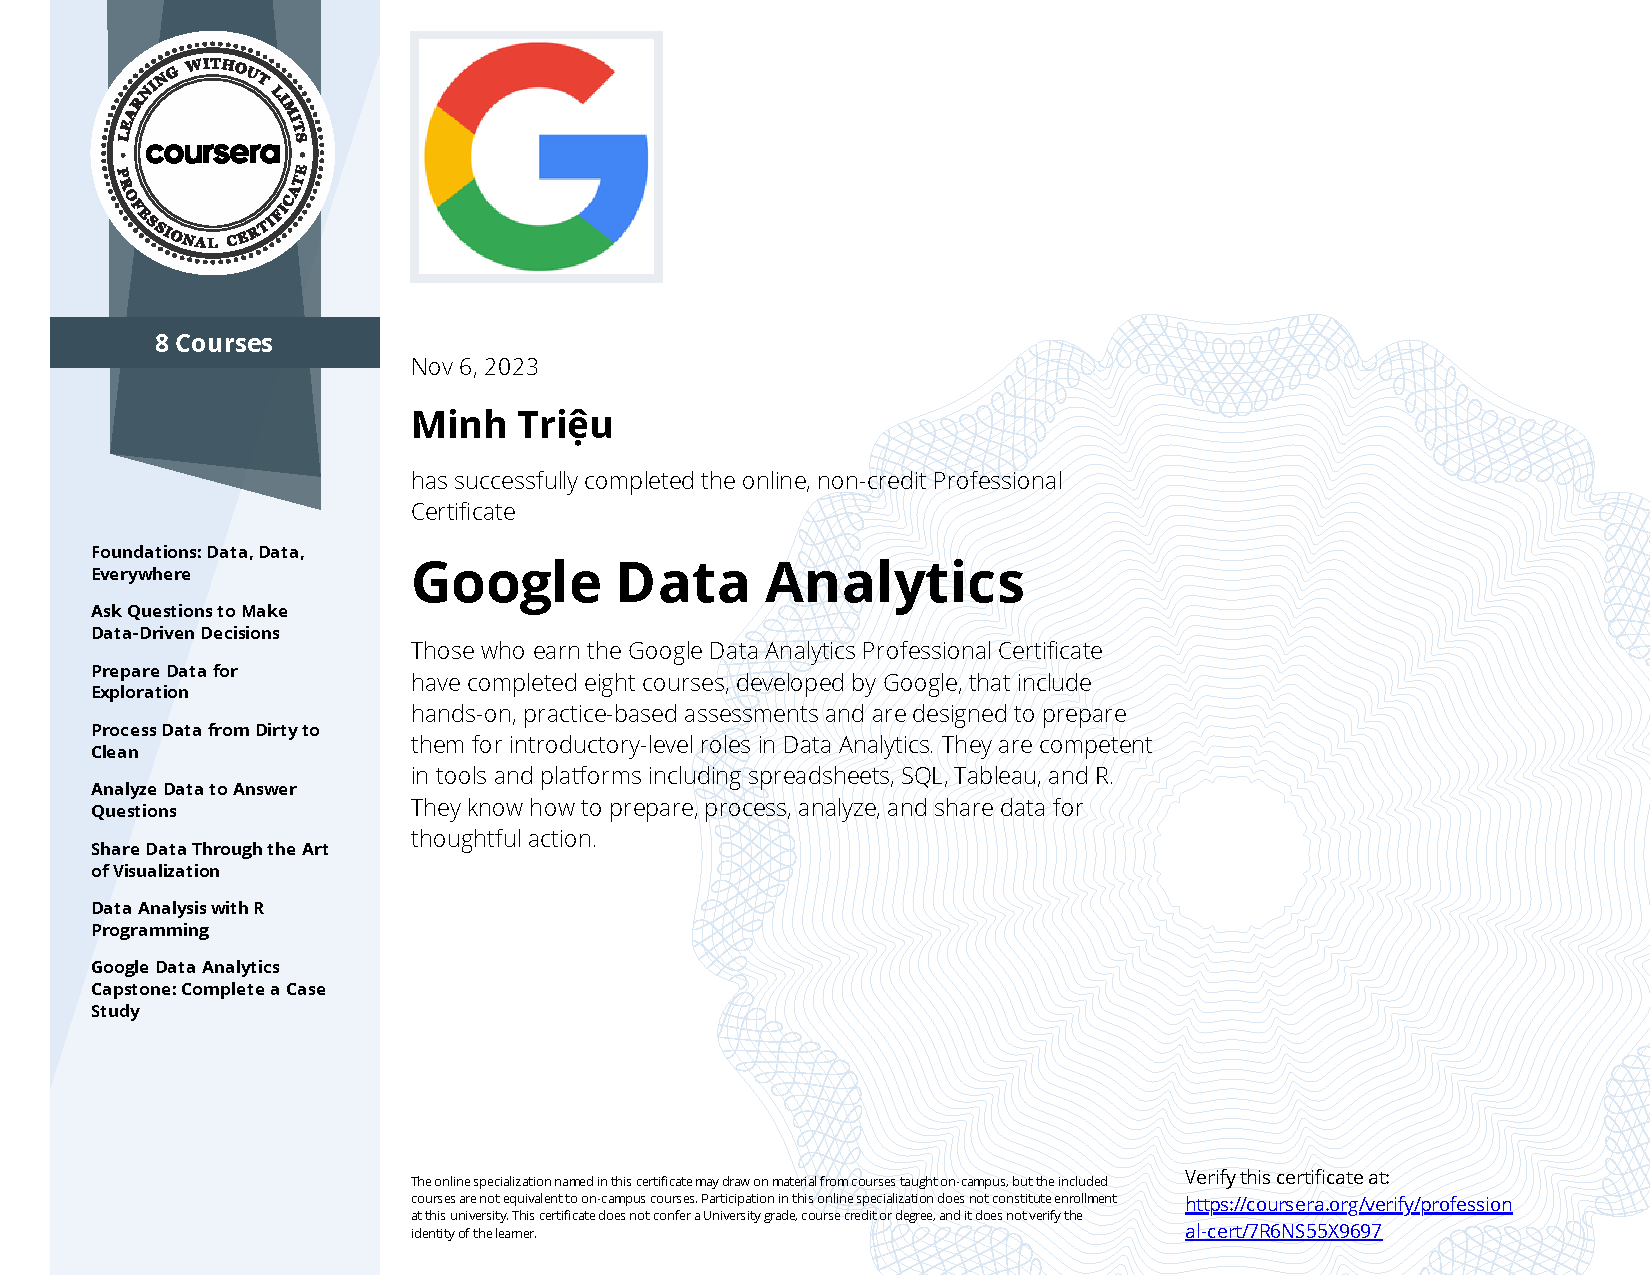
\includegraphics[width=\textwidth]{certs/7R6NS55X9697.pdf}
  \caption{\href{https://www.coursera.org/account/accomplishments/specialization/certificate/7R6NS55X9697}{Verification}}
\end{figure}

\subsection{Enrollment date (8 courses)}
\begin{enumerate}
  \item \href{https://www.coursera.org/account/accomplishments/certificate/S9CWWMGFJAMM}{Foundations: Data, Data, Everywhere - 22nd October 2023}
  \item \href{https://www.coursera.org/account/accomplishments/certificate/ZA7TH6KEEEPB}{Ask Questions to Make Data-Driven Decisions - 24th October 2023}
  \item \href{https://www.coursera.org/account/accomplishments/certificate/B7PZ38G3U9XR}{Prepare Data for Exploration - 27th October 2023}
  \item \href{https://www.coursera.org/account/accomplishments/certificate/DYHS63889XUN}{Process Data from Dirty to Clean - 29th October 2023}
  \item \href{https://www.coursera.org/account/accomplishments/certificate/6478SYGTR4HF}{Analyze Data to Answer Questions - 5th November 2023}
  \item \href{https://www.coursera.org/account/accomplishments/certificate/8JULNPUM3GLC}{Share Data Through the Art of Visualization - 6th November 2023}
  \item \href{https://www.coursera.org/account/accomplishments/certificate/JPHDNMYYDJZ9}{Data Analysis with R Programming - 6th November 2023}
  \item \href{https://www.coursera.org/account/accomplishments/certificate/7TN58662AD9X}{Google Data Analytics Capstone: Complete a Case Study - 6th November 2023}
\end{enumerate}
Completion date of each course: On certificate verification link.

\section{Course 1: Foundations: Data, Data, Everywhere}
I have gained a lot of knowledge from the course. It has taught me how to turn data into insights and comprehend the data ecosystem. I have also learned how to use data to make informed business decisions.
In module 2, I have developed my data analyst skills and practiced analytical thinking. I have learned how to define outcomes and how to measure them. I have also learned how to formulate good questions and communicate effectively with data.\par
In module 3, I have followed the data life cycle and described the data analysis process. I have learned about the data analysis toolbox and how to apply different tools for different tasks. I have also learned how to clean, explore, analyze, and interpret data.\par
In module 4, I have mastered spreadsheet basics and SQL. I have learned how to manipulate, query, and join data using spreadsheets and SQL. I have also learned how to plan a data visualization and select the right chart type for my data.\par
In module 5, I have explored data analyst job opportunities and the importance of fair business decisions. I have learned how to prepare for a data analyst interview and showcase my portfolio. I have also learned how to avoid bias and ensure ethical use of data. This course has provided me with a solid foundation for becoming a data analyst. I have learned how to use data to make informed business decisions. I have also learned how to use spreadsheets and SQL for data analysis.\par
About module challenges and course challenge, I find them very interesting and useful. They have helped me to practice my data analyst skills and apply what I have learned in the course. The instructor emphasizes the importance of asking questions and not making assumptions in data analysis work. He shared a story about an analyst who initially struggled because he was afraid to ask questions, but improved significantly once he started doing so.

\section{Course 2: Ask Questions to Make Data-Driven Decisions}
In the first module, I've gained knowledge on how to leverage data as a problem-solving tool and the art of formulating effective questions to guide my analysis. Furthermore, I've been introduced to the six stages of data analysis: ask, prepare, process, analyze, share, and act and acknowledged. I've also learned that data analysts commonly deal with six types of problems: making predictions, classifying things, detecting anomalies, identifying themes, uncovering relationships, and recognizing patterns.\par

In the second module, I've learned how to effectively communicate my findings through clear and engaging visuals. I've understood the difference between data and metrics, and how to choose the right metrics for my analysis. I've also gained knowledge on how to design compelling dashboards that can summarize my data, highlight key insights, and tell a story. Through practice quizzes, I've tested my knowledge on following the evidence and designing dashboards. The final task of the module helped me assess my understanding of the content and my ability to connect the data dots. Overall, this module has significantly enhanced my skills in data visualization and communication.\par

The third module taught me how to work with spreadsheets, which are essential tools for data analysis. It showed me how to use formulas and functions to perform calculations and manipulate data. It also demonstrated how to save time with structured thinking by using tables, filters, sorting, and conditional formatting. Even though I had used spreadsheets before, I learned many new things from this module. For instance, I used to struggle with the VLOOKUP function, but now, thanks to the hands-on activity, I can use it with ease.\par

The fourth module enhanced my data analyst communication skills. I learned to present data analysis results clearly using suitable visualizations and language. I practiced tailoring my messages to different audiences and responding to various data scenarios. The module also taught me to balance project expectations by setting SMART objectives, defining scope and deliverables, and transparently communicating progress and challenges. I learned to handle the tradeoff between speed and accuracy in data analysis, understanding data uncertainties and limitations.\par

\section{Course 3: Prepare Data for Exploration}

In the first module of Course 3, I delved into the world of data types and structures. This module equipped me with the ability to differentiate between structured and unstructured data, identify suitable data formats for various analytical needs, and extract pertinent information from diverse data sources.

The second module was a deep dive into the critical aspects of bias, credibility, privacy, ethics, and access in data. This module honed my critical thinking and ethical awareness, enabling me to handle data responsibly. I can now identify and circumvent bias in data collection and analysis, ensure the credibility of my data sources, and apply data ethics and privacy principles to safeguard the rights of data owners and users. The concept and practice of open data were also explored, providing me with a comprehensive understanding of its benefits and limitations.

In the third module, I gained hands-on experience with databases. I learned about fundamental database concepts and terminology, such as tables, records, fields, keys, and queries. I can now use various tools and methods, including SQL, filters, and sorting techniques, to access and extract data from databases. The importance and role of metadata in data analysis and documentation were also emphasized.

The fourth module focused on best practices and techniques for data organization and security. I learned to use consistent and meaningful naming conventions for my data files and folders, organize them logically, and employ various strategies and tools to protect my data from unauthorized access or loss, including passwords, encryption, backups, and cloud storage.

In the optional fifth module, I expanded my online presence and network as a data professional. I learned to manage my online profile on various platforms, such as LinkedIn, GitHub, Kaggle, and connect with other data professionals through online communities, forums, and events. I also learned how to showcase my skills and achievements through portfolios, projects, and certificates.

Finally, in the course challenge, I applied the knowledge and skills I acquired throughout the course to answer questions and solve problems in two real-world scenarios. This practical application of my learning helped me consolidate my understanding and gain confidence in my data preparation and exploration skills.

\section{Course 4: Process Data from Dirty to Clean}
Throughout this course, I learned various skills and techniques related to data processing, which is essential for effective data analysis. The first module covered the topic of data integrity, which refers to the accuracy and consistency of data. I learned how to check and ensure data integrity using different methods and tools, such as dealing with missing data. I also learned about the factors that affect the quality of data, such as sample size, sample bias, and random sampling.

The second module focused on the concept of clean data, which is data that is free of errors and inconsistencies. I learned how to identify and fix common data quality issues using spreadsheets and other software. This module helped me understand the benefits of clean data for analysis.

The third module taught me how to use SQL for data cleaning. I learned how to write SQL queries and functions to clean and transform data from databases. This module enhanced my data cleaning skills and made me more proficient in using SQL.

The fourth module showed me how to verify and report the results of data cleaning. This step is important in the data analysis process as it confirms that the data is ready for further analysis. I learned how to check that the data is clean and how to communicate the results of the data cleaning process effectively.

The optional module helped me prepare for the job market by teaching me how to add data to my resume. I learned about the job application process and how to create a resume that showcases my skills and experience. This module was very helpful in getting me ready for future opportunities.

The course ended with a Course Challenge, which tested my knowledge and skills from the course. The challenge gave me the chance to apply what I learned to realistic scenarios. It reinforced my understanding of the concepts and boosted my confidence in my data processing abilities.
\section{Course 5: Analyze Data to Answer Questions}
In the initial phase of Course 5, I learned about the importance of organizing data to facilitate analysis. I explored how to sort and filter data in both spreadsheets and SQL queries, and how to use temporary tables to organize data in SQL. This module emphasized the importance of well-organized data in efficient and effective analysis.

The next part of the course focused on formatting and adjusting data. I learned how to convert and format data, and how to use SQL queries to combine data. This module also highlighted the value of feedback and support from colleagues, showing me how collaboration can lead to new insights and improvements in my work.

The course then moved on to data aggregation. I explored various functions, procedures, and syntax to combine or aggregate data. I learned how to combine data within multiple cells in spreadsheets and within multiple database tables using SQL queries. This part of the course expanded my understanding of how to manipulate data to gain insights and achieve business objectives.

In the subsequent module, I delved into data calculations, a common task for data analysts. I learned about formulas, functions, and pivot tables in spreadsheets and SQL queries, all of which are used in data calculations. I also learned about the benefits of using SQL to manage temporary database tables.

Finally, the course concluded with a Course Challenge. This challenge allowed me to apply the key concepts I learned throughout the course. It tested my understanding of the material and gave me the opportunity to put theory into practice through three real-world scenarios. This final step helped consolidate my learning and gave me confidence in my data analysis skills.

\section{Course 6: Share Data Through the Art of Visualization}
Course 6 taught me the essential skills of data visualization, from the basics to the advanced. I started by learning the concepts of data visualization, such as accessibility, design thinking, and other factors that affect how data is perceived and understood. This module gave me a strong foundation for creating meaningful and accessible data visualizations.

Next, I learned how to use Tableau for data visualization. I explored the features and functions of Tableau and how they can help me create effective data visualizations. This module also helped me develop my creativity and clarity in visualizing data, enabling me to present my findings in a clear and engaging way.

Then, I learned how to tell stories with data. I learned how to identify the attributes of data-driven stories and how to link my objectives with my data through insights. I also practiced using Tableau to create dashboards and dashboard filters, which improved my data visualization skills.

After that, I learned how to create presentations and slideshows to communicate my data analysis. I learned how to consider all aspects of my analysis when creating a presentation and how to use multiple data sources in my visualizations. I also learned how to anticipate potential limitations and questions from stakeholders and how to provide useful answers.

Finally, I completed the Course Challenge. This challenge allowed me to apply what I learned throughout the course. It assessed my understanding of the material and gave me the chance to use theory in practice through two real-world scenarios. This final step consolidated my learning and gave me confidence in my data visualization skills.

\section{Course 7: Data Analysis with R Programming}
The first module of Course 7 familiarized me with the basics of R and RStudio. R is a programming language that specializes in data analysis, and RStudio is an integrated development environment (IDE) that improves the user experience of R. This section of the course showed me the advantages of using RStudio and how it can enhance the capabilities and features of R.

The following section of the course taught me how to program using RStudio. I learned about the essential concepts of R, such as functions and variables that can be used for computations and other programming tasks. I also learned about R packages, which are sets of R functions, code, and sample data that can be used in RStudio.

The course then proceeded to working with data in R. I learned how R can help manipulate, organize, and clean data through functions and other processes. I learned about data frames and how to handle them in R. I also revisited the idea of data bias and how R can be used to mitigate it.

In the next module, I learned about creating elaborate visualizations using R. I learned how to create and troubleshoot visualizations, enhance the appearance of visualizations, annotate visualizations, and save changes.

The course then explored documentation and reports. I examined R Markdown, a file format for creating dynamic documents with R. I learned how to format and export R Markdown documents and how to embed R code chunks into these documents.

Finally, the course ended with a Course Challenge. This challenge enabled me to apply the main principles I learned throughout the course. It assessed my comprehension of the material and gave me the chance to put theory into practice through three real-world scenarios. This final step reinforced my learning and gave me confidence in my R programming skills.

\section{Course 8: Google Data Analytics Capstone: Complete a Case Study}
\begin{itemize}
  \item
\end{itemize}
\section{Conclusion}
\begin{itemize}
  \item
\end{itemize}
\end{document}